\section{Mege Binary Insertion Sort implementation}
\section{Introduction}
The purpose of this report is to provide the tests that have been done to find the best value of K for the Merge Binary Insertion Sort algorithm.
Considering that Merge Binary Insertion Sort is a hybrid algorithm that has ability to handle large input and for its speed, but it became inefficient when having a small input, in the case of small input the library switch to Binary Insertion sort, that is more efficient on small input.

\section{Testing methodolgy}
To test the algorithm, I used a bash script\footnote{All the test are done on a Lenovo Thinkpad x390 yoga with an Intel Core i7-8665U and 16 gb of ram} that run the program with different values of K and for each field to sort, saving the time and the value of the algorithm parameter K.

\subsection{Some graphs}
\begin{figure}[H]
  \centering
    \caption{Time used to sort string field with different K values}
  \begin{minipage}{.45\textwidth}
    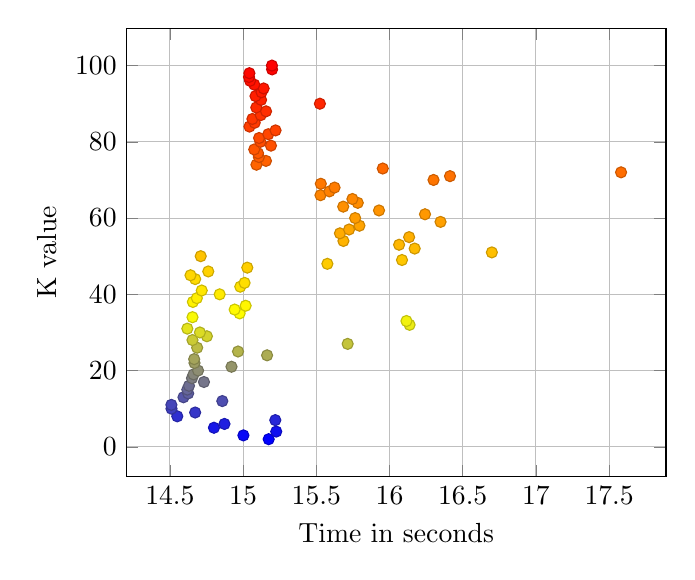
\begin{tikzpicture}
      \begin{axis}[
        ylabel={K value},
        xlabel={Time in seconds},
        grid=major,
        legend pos=north west,
      ]
    
      % Add your data points here
      % The 'nan' values indicate that the algorithm did not terminate for those max_height values
      \addplot+[
        scatter,
        only marks,
        error bars/.cd,
        y dir=both,
        y explicit,
        error bar style={line width=1pt},
      ] table[
        x index=0,  % Use the first column as x
        y index=1,  % Use the second column as y
        col sep=comma,
      ] {
        x, y
        nan, 2
        nan, 3
        nan, 4
        nan, 5
15.174793,2
15.002120,3
15.226469,4
14.801018,5
14.872827,6
15.219994,7
14.550677,8
14.672743,9
14.511134,10
14.510299,11
14.858102,12
14.592909,13
14.625006,14
14.619163,15
14.630402,16
14.732755,17
14.650927,18
14.661558,19
14.692577,20
14.920891,21
14.668250,22
14.665938,23
15.164005,24
14.965444,25
14.686458,26
15.714101,27
14.654403,28
14.752893,29
14.705142,30
14.619236,31
16.137131,32
16.115663,33
14.654513,34
14.976515,35
14.942336,36
15.017492,37
14.657133,38
14.684382,39
14.840178,40
14.717586,41
14.980832,42
15.010200,43
14.672827,44
14.640912,45
14.762319,46
15.028782,47
15.575648,48
16.085255,49
14.710605,50
16.698920,51
16.171816,52
16.065489,53
15.685135,54
16.133955,55
15.661422,56
15.723801,57
15.794644,58
16.348417,59
15.765204,60
16.242324,61
15.928335,62
15.683911,63
15.783138,64
15.746582,65
15.528558,66
15.589543,67
15.624654,68
15.530848,69
16.300621,70
16.413081,71
17.581432,72
15.953920,73
15.091242,74
15.156222,75
15.107862,76
15.102240,77
15.076253,78
15.190217,79
15.118428,80
15.109305,81
15.172208,82
15.221578,83
15.043744,84
15.079376,85
15.063591,86
15.120637,87
15.156885,88
15.090205,89
15.524503,90
15.122923,91
15.084973,92
15.125978,93
15.140413,94
15.076556,95
15.047903,96
15.040355,97
15.043084,98
15.198039,99
15.197005,100
      };
    
      \end{axis}
    \end{tikzpicture}
  \end{minipage}%
    \caption{Time used to sort integer field with different K values}
  \begin{minipage}{.45\textwidth}
    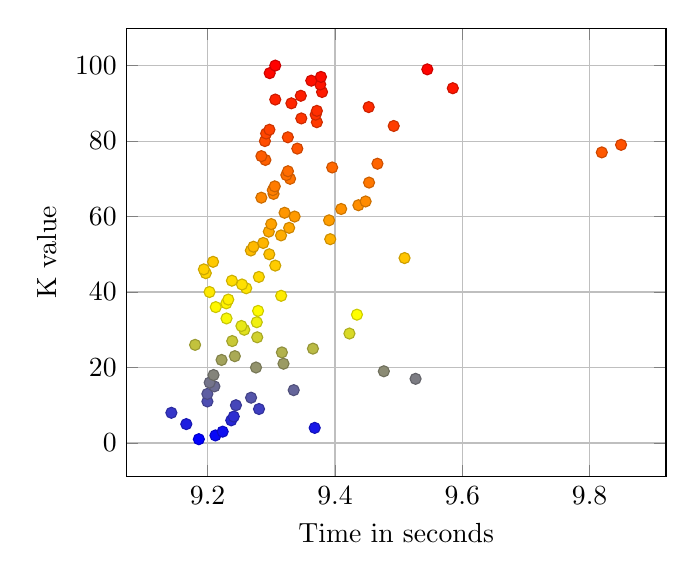
\begin{tikzpicture}
      \begin{axis}[
        ylabel={K value},
        xlabel={Time in seconds},
        grid=major,
        legend pos=north west,
      ]
    
      % Add data for the second graph here
      \addplot+[
        scatter,
        only marks,
        error bars/.cd,
        y dir=both,
        y explicit,
        error bar style={line width=1pt},
      ] table[
        x index=0,
        y index=1,
        col sep=comma,
      ] {
        9.186197,1
9.212261,2
9.223599,3
9.368176,4
9.166494,5
9.237125,6
9.241028,7
9.143051,8
9.280712,9
9.244462,10
9.199643,11
9.268249,12
9.199577,13
9.335217,14
9.210641,15
9.203176,16
9.526607,17
9.209284,18
9.476788,19
9.275986,20
9.319157,21
9.221870,22
9.242745,23
9.316632,24
9.365391,25
9.180305,26
9.238643,27
9.277911,28
9.422732,29
9.257569,30
9.253060,31
9.277205,32
9.229656,33
9.434564,34
9.279232,35
9.212737,36
9.229342,37
9.232473,38
9.315504,39
9.202983,40
9.260608,41
9.253942,42
9.238150,43
9.280483,44
9.197095,45
9.194084,46
9.306260,47
9.208529,48
9.509313,49
9.296849,50
9.267894,51
9.271972,52
9.287302,53
9.392591,54
9.315284,55
9.296102,56
9.328053,57
9.299902,58
9.390757,59
9.336653,60
9.320850,61
9.409764,62
9.436843,63
9.448167,64
9.284360,65
9.303523,66
9.302370,67
9.305449,68
9.453555,69
9.329503,70
9.323660,71
9.326175,72
9.395645,73
9.466731,74
9.290731,75
9.284439,76
9.819143,77
9.340883,78
9.849433,79
9.289960,80
9.325991,81
9.291882,82
9.297047,83
9.492295,84
9.371555,85
9.347150,86
9.369679,87
9.371593,88
9.452995,89
9.331566,90
9.306230,91
9.346358,92
9.379721,93
9.585127,94
9.376938,95
9.362821,96
9.377997,97
9.297483,98
9.545093,99
9.306211,100
      };
    
      \end{axis}
    \end{tikzpicture}
  \end{minipage}%
    \caption{Time to sort double field with different K values}
  \begin{minipage}{.45\textwidth}
    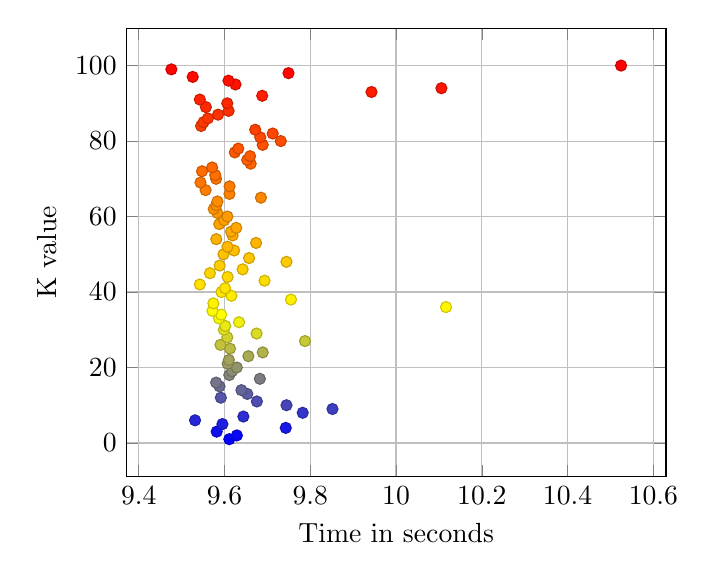
\begin{tikzpicture}
      \begin{axis}[
        ylabel={K value},
        xlabel={Time in seconds},
        grid=major,
        legend pos=north west,
      ]
    
      % Add data for the third graph here
      \addplot+[
        scatter,
        only marks,
        error bars/.cd,
        y dir=both,
        y explicit,
        error bar style={line width=1pt},
      ] table[
        x index=0,
        y index=1,
        col sep=comma,
      ] {
        9.611292,01
9.628809,02
9.581890,03
9.742901,04
9.595193,05
9.531385,06
9.644048,07
9.782362,08
9.851846,09
9.744601,10
9.675519,11
9.591549,12
9.653216,13
9.639436,14
9.588447,15
9.580535,16
9.682539,17
9.611242,18
9.617495,19
9.628731,20
9.607388,21
9.610234,22
9.655736,23
9.689200,24
9.612920,25
9.590629,26
9.787650,27
9.606557,28
9.674862,29
9.598662,30
9.601851,31
9.633987,32
9.587216,33
9.592257,34
9.571808,35
10.116558,36
9.574109,37
9.755062,38
9.616204,39
9.592911,40
9.601447,41
9.542522,42
9.693356,43
9.607328,44
9.566053,45
9.642313,46
9.588713,47
9.744500,48
9.657336,49
9.597604,50
9.622466,51
9.606987,52
9.673616,53
9.580895,54
9.619047,55
9.615345,56
9.627492,57
9.587838,58
9.599259,59
9.606814,60
9.582998,61
9.574987,62
9.580574,63
9.583611,64
9.684982,65
9.611648,66
9.555973,67
9.611889,68
9.544073,69
9.580480,70
9.578523,71
9.547654,72
9.571253,73
9.661080,74
9.652991,75
9.659703,76
9.624139,77
9.632183,78
9.689063,79
9.731268,80
9.683407,81
9.712429,82
9.671672,83
9.545444,84
9.551162,85
9.561359,86
9.585052,87
9.609620,88
9.556609,89
9.606460,90
9.542524,91
9.687990,92
9.942815,93
10.105839,94
9.625593,95
9.609298,96
9.525934,97
9.749306,98
9.476184,99
10.524733,100
      };
    
      \end{axis}
    \end{tikzpicture}
  \end{minipage}
\end{figure}

\section{Conclusion based on the analysis}
As we can see from the graphs, the optimal values for k is around 10 and 20, and the fact that based on the actual implementation is also important the type of field that the algorithm is sorting.
In fact when sorting integer or double the algorithm is taking way less time than sorting string, probably caused by miss branch prediction. 
Also in the graph we can see some outliers, this can be caused by bottleneck of other processes or just the fact that the laptop in some point was charging.

